\documentclass{article}
\usepackage{fontspec}
\usepackage{graphicx}
\usepackage{fancyhdr}
\usepackage{geometry}
\usepackage{lipsum}
\usepackage[spanish]{babel}
\usepackage{xcolor}
\usepackage{eso-pic}
\usepackage{tikz}
\usepackage{atbegshi}
\usepackage[most]{tcolorbox} 
\usepackage{listings}
\usepackage{fontawesome5}

\usetikzlibrary{backgrounds}

\setmainfont[
    Path = ./fonts/Poppins/,
    Extension = .ttf,
    UprightFont = *-Regular.ttf,
    BoldFont = *-Bold.ttf,
    ItalicFont = *-Italic.ttf,
    BoldItalicFont = *-BoldItalic.ttf,
    % LetterSpace=5, 
]{Poppins}



\newlength{\borderwidth}
\setlength{\borderwidth}{20pt} 


\geometry{a4paper,
          left=\dimexpr1cm+\borderwidth,
          right=\dimexpr1cm+\borderwidth,
          top=\dimexpr2cm+\borderwidth,
          bottom=\dimexpr0.5cm+\borderwidth,
          headheight=1.5cm,
          headsep=0.5cm}


\pagestyle{fancy}
\fancyhf{}
\fancyhead[L]{\raisebox{0\height}{
\includegraphics[height=1cm,keepaspectratio]{logo-header.png}}}
\fancyhead[R]{\raisebox{1.25\height}{\large\textbf{Academia Juvenil de Programación Competitiva}}}
\renewcommand{\headrulewidth}{0pt}


\definecolor{primary}{HTML}{116BB1}
\definecolor{secondary}{HTML}{711E8C}
\definecolor{tertiary}{HTML}{1ECA6C}


\newcommand{\borderOverlay}{
    \begin{tikzpicture}[remember picture, overlay]
        \draw[line width=\borderwidth, color=primary]
            (current page.north west) -- 
            (current page.north east) --
            (current page.south east) --
            (current page.south west) -- cycle;
    \end{tikzpicture}
}

\AddToShipoutPictureBG{\borderOverlay}

\newtcolorbox{container}[1]{ 
    colback=white, 
    colframe=primary,
    coltitle=white,
    title={#1},
    fonttitle=\bfseries, 
    arc=2pt,
    boxrule=2pt, 
    enhanced, 
    breakable, 
    attach boxed title to top left={xshift=5pt, yshift=-5pt}, 
    boxed title style={colback=primary, size=small}, 
}


\lstdefinestyle{cppstyle}{
    language=C++,
    basicstyle=\ttfamily\small,
    keywordstyle=\color{primary},
    commentstyle=\color{tertiary},
    stringstyle=\color{secondary},
    backgroundcolor=\color{white!100},
    breaklines=true,
    breakatwhitespace=true,
    tabsize=4,
    showstringspaces=false,
    captionpos=b
}

\newcommand{\cppfile}[2][]{
    \begin{container}{\faCode \space \space  #1}
        \lstinputlisting[style=cppstyle]{#2}
    \end{container}
}

\newcommand{\inlinecpp}[1]{
    \lstinline[
        language=C++,
        basicstyle=\ttfamily\small\color{primary!80!black},
        keywordstyle=\color{primary},
        stringstyle=\color{secondary},
        commentstyle=\color{tertiary}
    ]|#1|
}


\newcommand{\documentTitle}{Clase 2}
\newcommand{\documentSubtitle}{Contenidos y ejercicios prácticos}
\newcommand{\documentAuthor}{Francisco Muñoz}
\newcommand{\documentDate}{\today}

\begin{document}

\thispagestyle{empty}
\AddToShipoutPictureBG*{}
\begin{center}
    \vspace*{2cm}
    
\includegraphics[width=0.75\textwidth]{logo.png} \\[1.5cm]
    {\Huge \textbf{\documentTitle}} \\[0.5cm]
    {\Large \documentSubtitle} \\[1.5cm]
    {\large \documentAuthor} \\[0.5cm]
    {\large \space \space \documentDate}
    \vfill
    {\large Academia Juvenil de Programación Competitiva}
\end{center}
\newpage

\section{Introducción}

Este documento contiene los contenidos que deberían ser vistos durante la \textbf{Clase N°2}, además de contener ejercicios prácticos.

\section{Índice}

\begin{itemize}
    \item Contenidos
    \begin{itemize}
        \item Variables
        \item Operando con variables
        \item Estructura de un problema de programación competitiva
        \item cout y cin
    \end{itemize}
    \item Ejercicios Prácticos
\end{itemize}

\section{Contenidos}

\subsection{Variables}

\textbf{¿Qué es una variable?}

Una variable es un espacio de memoria reservado para almacenar un dato que puede cambiar durante la ejecución de un programa. En C++, cada variable debe tener un tipo definido, que indica qué clase de datos puede almacenar (por ejemplo, enteros, caracteres, booleanos, etc.).

\textbf{Declaración de variables:}

Para declarar una variable, se debe especificar el tipo de dato seguido del nombre de la variable, \textbf{no es necesario} definirle un valor. Ejemplos:


\cppfile[Ejemplo]{codes/definir.cpp}

\textbf{Inicialización de variables:}

Para \textbf{iniciailzar} una variable hay que asignarle un valor al momento de declararla:

\cppfile[Ejemplo]{codes/variables1.cpp}


\textbf{Reglas para nombrar variables:}
\begin{itemize}
    \item Deben comenzar con una letra o guión bajo.
    \item Pueden contener letras, números y guión bajo.
    \item No pueden ser palabras reservadas del lenguaje.
    \item Se recomienda usar nombres descriptivos.
\end{itemize}

\subsection{Operando con variables}

Las variables pueden ser utilizadas para realizar operaciones, asignaciones y comparaciones. A continuación, algunos ejemplos básicos:

\textbf{Operaciones aritméticas:}

\cppfile[Ejemplo]{codes/variables2.cpp}

\textbf{Operaciones con flotantes:}

\cppfile[Ejemplo]{codes/variables3.cpp}

\textbf{Concatenación de cadenas:}

\cppfile[Ejemplo]{codes/variables4.cpp}


\subsection{Estructura de un problema de programación competitiva}

Los problemas de programación competitiva suelen tener una estructura estándar. Comprender esta estructura es esencial para poder interpretar correctamente los enunciados y resolver los problemas eficientemente.

\begin{itemize}
    \item \textbf{Statement (Enunciado):} Es la descripción del problema. Suele presentar una situación (a veces con una historia) y definir claramente qué se pide. Puede incluir ejemplos o explicaciones del objetivo principal.
    
    \item \textbf{Input (Entrada):} Describe qué datos se entregarán al programa. Se especifica el número y tipo de datos que serán leídos desde la entrada estándar (\texttt{cin} en C++).

    \item \textbf{Output (Salida):} Especifica el formato y contenido que debe tener la salida del programa. Los datos deben ser impresos exactamente como se indica (usando \texttt{cout} en C++), respetando espacios, saltos de línea y el orden.

    \item \textbf{Constraints (Restricciones):} Define los límites que tendrán los datos de entrada. Por ejemplo, puede decir que $1 \leq n \leq 10^5$, lo que te permite saber qué tan eficiente debe ser tu solución.

    \item \textbf{Notes (Notas):} A veces se entregan aclaraciones adicionales, explicaciones de los ejemplos o situaciones límite a considerar.

    \item \textbf{Test Cases (Casos de prueba):} Son ejemplos concretos de entradas y salidas. Se utilizan para entender cómo debe funcionar el programa en la práctica.
\end{itemize}

\vspace{0.5cm}

\begin{center}
    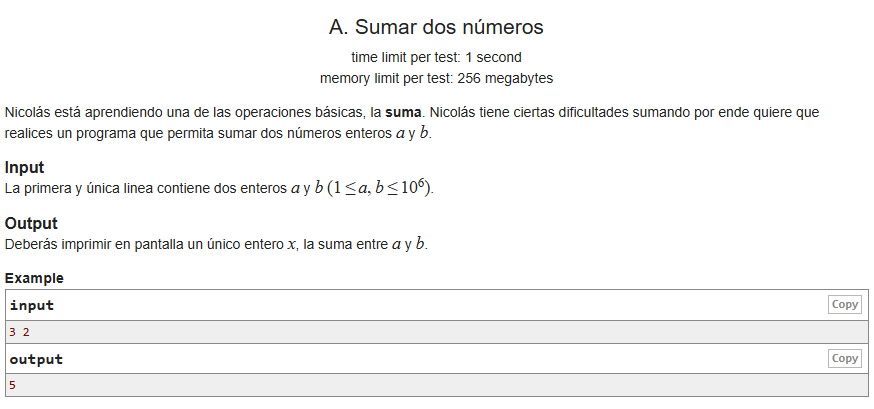
\includegraphics[width=0.8\textwidth]{img/statementexample.png}
    
    \textit{Ejemplo de problema con estructura clásica.}
\end{center}

\vspace{0.5cm}

\textbf{Consejo:} Antes de programar, es muy útil subrayar o anotar qué tipo de datos se están leyendo y qué se espera imprimir. También es clave observar los límites (constraints) para decidir si se necesita una solución eficiente.


\cppfile[Ejemplo de Solución]{codes/ejemplosuma.cpp}

\vspace{0.5cm}


\textbf{Consejos:}
\begin{itemize}
    \item Siempre usar \texttt{int main()} con \texttt{return 0;} al final.
    \item Leer con \texttt{cin} y escribir con \texttt{cout}.
    \item Prestar atención al formato de salida pedido por el enunciado.
\end{itemize}

\subsection{cout y cin}

\texttt{cout} y \texttt{cin} son objetos de entrada/salida en C++ definidos en la biblioteca \texttt{iostream}.

\vspace{1.5cm}


\textbf{cout:} Se usa para imprimir información en pantalla.



\cppfile[Ejemplo]{codes/cout.cpp}

\textbf{cin:} Se usa para leer datos desde la entrada estándar (el teclado).

\cppfile[Ejemplo]{codes/cinex.cpp}

\textbf{Múltiples entradas/salidas:}

\cppfile[Ejemplo]{codes/meys.cpp}

\textbf{Notas adicionales:}
\begin{itemize}
    \item \texttt{endl} se utiliza para insertar un salto de línea.
    \item También se puede usar \texttt{\textbackslash n} para hacer lo mismo.
    \item Es importante respetar el orden de las variables en \texttt{cin} y \texttt{cout}.
\end{itemize}

\section{Ejercicios Prácticos}


\begin{container}{Problema 1 - Suma Básica}
Escribe un programa que reciba dos enteros y devuelva su suma.   
\end{container}

\textbf{Input}

El programa recibe dos enteros $a$ y $b$, separados por un espacio. ($-1000 \leq a, b \leq 1000$)

\vspace{0.5em}
\textbf{Output}

Un solo número: la suma de $a$ y $b$.

\vspace{0.5em}

\begin{container}{Ejemplo - Input}
5 3
\end{container}

\begin{container}{Ejemplo - Output}
8
\end{container}

\vspace{3.5em}


\begin{container}{Problema 2 – mapache azul o azul mapache}
Dadas dos cadenas de texto en un orden \texttt{texto1} \texttt{texto2}, escribe un programa que invierta su orden, es decir, el nuevo orden es \texttt{texto2} \texttt{texto1}.
\end{container}

\textbf{Input}
Dos cadenas de texto $a$ y $b$.

\vspace{0.5em}
\textbf{Output}
Las dos cadenas de texto en el orden $b$ $a$.


\vspace{0.5em}

\begin{container}{Ejemplo - Input}
mapache azul
\end{container}


\begin{container}{Ejemplo - Output}
azul mapache
\end{container}

\vspace{3.5em}



\begin{container}{Problema 3 – La concatenación extraña}
Escribe un programa que reciba dos cadenas de texto y las una en una sola.
\end{container}


\textbf{Input}

Dos líneas. Cada una contiene una palabra (sin espacios).

\vspace{0.5em}
\textbf{Output}

Una línea con la palabra unida.

\vspace{0.5em}

\begin{container}{Ejemplo - Input}
hola\\
mundo
\end{container}

\begin{container}{Ejemplo - Output}
holamundo
\end{container}

\vspace{3.5em}


\begin{container}{Problema 4 – Suma y resta}
Escribe un programa que reciba dos números $a$ y $b$ ($1 \leq a,b \leq 20$). El programa deberá imprimir la suma y la resta de ambos números.
\end{container}

\textbf{Input}

Dos números naturales en la primera línea separados por un espacio.

\vspace{0.5em}
\textbf{Output}

El output consiste en dos líneas. La primera corresponde a un único entero: la \textbf{suma} de los enteros $a$ y $b$.
La segunda línea corresponde a un único entero: la \textbf{resta} de los enteros $a$ y $b$.

\vspace{0.5em}

\begin{container}{Ejemplo - Input}
5 4
\end{container}

\begin{container}{Ejemplo - Output}
9
1
\end{container}



\end{document}